\documentclass[11pt]{article}

% Typography and page geometry match bfs-avoidance-frontier/paper/main.tex.
\usepackage[margin=1.1in]{geometry}
\usepackage[T1]{fontenc}
\usepackage{microtype}
\usepackage{amsmath,amssymb,amsthm}
\usepackage{booktabs,longtable,array}
\usepackage{graphicx}
\usepackage{flafter}
\usepackage{placeins}
\newcolumntype{L}[1]{>{\raggedright\arraybackslash}p{#1}}
\usepackage{enumitem}
\usepackage{xurl}
\usepackage[hidelinks]{hyperref}
\hypersetup{
 pdftitle={An Empirical Evaluation of Message Delivery Reliability and Recovery Characteristics in Redis Streams and NATS JetStream},
 pdfauthor={Victor Bona},
 pdfsubject={Reproducible evaluation of message recovery, concurrency, and persistence},
 pdfkeywords={Redis Streams, NATS JetStream, recovery, durability, consumer failure, empirical evaluation}
}
\newtheorem{theorem}{Theorem}[section]
\newtheorem{proposition}[theorem]{Proposition}
\newtheorem{corollary}[theorem]{Corollary}
\theoremstyle{definition}
\newtheorem{definition}[theorem]{Definition}
\newtheorem{remark}[theorem]{Remark}
\newcommand{\code}[1]{\texttt{#1}}
\newcommand{\artifact}[1]{\texttt{\path{#1}}}
\newcommand{\MainMessages}{4,915,200}
\newcommand{\TimedMessages}{12,434,648}
\newcommand{\SerialMessages}{61,440}
\newcommand{\KillBracket}{2.291}
\newcommand{\RedisMemorySpeedup}{12.59}
\newcommand{\RedisMemoryPubRate}{73.90}
\newcommand{\RedisMemoryPubPnn}{0.47}
\newcommand{\RedisPeriodicSpeedup}{11.02}
\newcommand{\RedisPeriodicPubRate}{61.38}
\newcommand{\RedisPeriodicPubPnn}{0.56}
\newcommand{\RedisAlwaysSpeedup}{8.59}
\newcommand{\RedisAlwaysPubRate}{3.03}
\newcommand{\RedisAlwaysPubPnn}{29.00}
\newcommand{\RedisSyncSlowdown}{24.4}
\newcommand{\NatsMemorySpeedup}{12.94}
\newcommand{\NatsMemoryPubRate}{60.38}
\newcommand{\NatsMemoryPubPnn}{0.70}
\newcommand{\NatsPeriodicSpeedup}{12.36}
\newcommand{\NatsPeriodicPubRate}{49.49}
\newcommand{\NatsPeriodicPubPnn}{0.85}
\newcommand{\NatsAlwaysSpeedup}{12.24}
\newcommand{\NatsAlwaysPubRate}{0.37}
\newcommand{\NatsAlwaysPubPnn}{579.57}
\newcommand{\NatsSyncSlowdown}{161.1}

\newcommand{\RedisAlwaysPnnMean}{29.0}
\newcommand{\RedisAlwaysPnnMedian}{7.5}
\newcommand{\RedisAlwaysPnnLooMin}{20.2}
\newcommand{\RedisAlwaysPnnLooMax}{32.1}
\newcommand{\NatsAlwaysPnnMean}{579.6}
\newcommand{\NatsAlwaysPnnMedian}{160.3}
\newcommand{\NatsAlwaysPnnLooMin}{150.5}
\newcommand{\NatsAlwaysPnnLooMax}{639.4}


\title{An Empirical Evaluation of Message Delivery Reliability and Recovery Characteristics in Redis Streams and NATS JetStream}
\author{Victor Bona\\[2pt]
\small Independent Researcher, Blumenau, Brazil\\
\small \texttt{victor.bona@hotmail.com}}
\date{September 2026}

\begin{document}
\maketitle
\begin{abstract}
Consumer-progress acknowledgments in Redis Streams and NATS JetStream have different persistence implications even under always-synchronize append policies. We evaluate that distinction alongside recovery timing, consumer concurrency and publication cost using single-replica deployments on a two-node Kubernetes homelab. The study compares Redis 7.4.2/8.10.2 and NATS Server 2.10.24/2.15.0, preserving an original campaign and adding three deployments with fresh broker processes and stores, matched publication durations, CPU sensitivity and storage diagnostics. All 240 active follow-up recovery episodes completed, including live, deliberately unacknowledging consumers; twelve plain Redis read controls remained pending. Receipt timing followed residual eligibility plus policy-dependent excess. Redis's integrated CLAIM path exhibited greater excess than the tested explicit reclamation loop in this quiet, one-message workload. Sixteen consumers increased current memory/periodic drain throughput by 10.43--14.49 times across deployment-specific comparisons, while cycle p99 increased and driver capacity affected rates. At sixteen publishers, current periodic/memory publication ratios averaged 0.8257 for Redis and 0.8207 for JetStream. Ten of 72 planned always-profile publication trials failed (13.9\%), including four warm-up failures, compared with one of 72 periodic trials and none of 72 memory trials. Timed failures returned five-second client timeouts with unknown confirmation outcomes. A compact analytical model and selected Lean-checked statements delimit the claims; full proofs and detailed results are included in the appendices. The licensed artifact retains timings, failures, configurations and reproducible analysis. These observations characterize specified policies and acknowledgment costs; they do not establish equal durability contracts, power-loss survival or hardware-independent rankings.
\end{abstract}


\noindent\textbf{Keywords:} message delivery; Redis Streams; NATS JetStream; consumer failure; redelivery latency; persistence; reproducible benchmarking.

\section{Introduction}\label{sec:intro}

A consumer can disappear after receiving a message but before acknowledging it. Recovering that message requires more than retaining its payload: the system must preserve the pending-delivery state, make the message eligible again, and supply it to an available consumer. The resulting delay depends on both broker policy and client behavior. Conversely, a fast acknowledgment can indicate acceptance without establishing that either a message or a consumer's progress has reached stable storage. These distinctions make a single throughput number an incomplete basis for selecting a messaging system.

Redis Streams and NATS JetStream expose different recovery policies and acknowledgment contracts. Redis consumer groups retain pending entries for explicit reclamation, including the integrated \code{XREADGROUP CLAIM} mechanism in current releases. JetStream tracks acknowledgment deadlines and supplies expired work when pull demand exists~\cite{redis742stream,redis8102stream,nats21024consumer,nats2150consumer}. Their ``always'' append settings also differ from a guarantee that each consumer acknowledgment synchronously persists consumer progress. A comparison must identify which operation and contract it measures.

This study asks three questions:
\begin{enumerate}[label=\textbf{RQ\arabic*:},leftmargin=3.5em]
\item How does consumer failure affect message redelivery latency?
\item How do both systems behave under increasing consumer concurrency?
\item What are the throughput/latency trade-offs under different durability configurations?
\end{enumerate}

We operationalize RQ1 as assessment of residual timeout and recovery-policy overhead, RQ2 as acknowledged backlog-drain scaling and driver-capacity sensitivity, and RQ3 as confirmed-publication cost under specified persistence settings. The contribution is the combination of explicit acknowledgment semantics, controlled recovery interventions, and reproducible observations. It is not a new general-purpose broker benchmark or a proof of implementation correctness.

The original single-deployment campaign evaluated Redis 7.4.2 and NATS Server 2.10.24 through 300 drain trials, 60 planned publication trials, 60 serial trials, 120 consumer kills, and ten controls. Its unequal storage-history carryover motivated a prospective follow-up: three newly provisioned deployments, fresh broker processes and stores for every trial, matched publication durations, phase-specific CPU observations, and synchronization traces. The follow-up also evaluates Redis 8.10.2 and NATS Server 2.15.0, and adds live, unacknowledging recovery controls. All workloads run on the same two-node Kubernetes homelab. Historical and follow-up observations remain separate datasets.

The analytical model establishes conditional identities, bounds, and counterexamples. Measurements establish the observed behavior of the specified workloads and client paths. Neither layer supplies a hardware-independent ranking or a tested stable-storage guarantee. The distinction allows each research question to receive a concrete answer without treating empirical regularities as universal theorems.

\section{Background and related work}\label{sec:background}

Delivery guarantees combine distinct safety and liveness claims. Retaining an unacknowledged message is a safety property; eventually assigning it to a live consumer additionally requires a recovery policy and progress assumptions. At-least-once delivery permits duplicates and does not establish exactly-once application effects. We distinguish publication confirmation, client receipt, broker processing of a consumer acknowledgment, and completion of an external effect~\cite{birrell1984,saltzer1984}. Persistence describes which state is intended to survive a stated failure class. A consumer-process failure, broker-process failure, pod deletion, and host power loss therefore cannot be treated as interchangeable tests of ``durability.''

\subsection{Redis Streams}

\code{XADD} appends an entry to a stream. With acknowledgment tracking enabled, \code{XREADGROUP} assigns an entry to a consumer and records it in the group's pending-entry list (PEL). \code{XACK} removes the corresponding pending record; it does not delete the stream entry~\cite{redisxreadgroup,redisxack}. A plain new-message read with \code{>} and no CLAIM option does not transfer another consumer's pending entries. Consequently, consumer death and message reassignment are separate events.

In Redis 7.4.2, \code{XAUTOCLAIM} scans pending entries and transfers those whose idle age reaches the configured minimum. It exposes a continuation cursor; a general reclaimer must advance that cursor and revisit the list. A call scans at most ten times its \code{COUNT} bound, so an arbitrary-size PEL cannot be treated as a single timer event~\cite{redisxautoclaim,redis742stream}. Our recovery experiment deliberately has one pending message and \code{COUNT}=1. This isolates timeout and polling behavior, but does not evaluate a large pending-list scan. Redis 8.10.2 additionally supports \code{XREADGROUP CLAIM}, which can consider eligible pending entries within a blocking group read~\cite{redis8102stream}. The follow-up compares that policy with \code{XAUTOCLAIM} on both releases. A plain \code{>} read without CLAIM still supplies no reclamation operation.

Redis persistence is configured separately from stream consumption. We disable snapshots and compare no append-only file (AOF), AOF with \code{appendfsync everysec}, and AOF with \code{appendfsync always}. The last setting can group commands into a shared synchronization operation; it need not issue one synchronization call per message. The nominal every-second mode does not prove a hard one-second power-loss window: the pinned implementations can postpone writes while a previous background synchronization is in progress, and I/O or scheduling delay remains possible~\cite{redispersistence,redis742aof,redis8102aof,redis742config}.

\subsection{NATS JetStream}

JetStream stores messages in streams and records delivery progress in consumers. We use one durable pull consumer shared by all workers, explicit per-message acknowledgment, no acknowledgment backoff, and one stream replica. Workers bind to this same consumer instead of creating independent durable consumers, which would represent separate subscriptions rather than competing workers~\cite{natsconsumers}.

\code{AckWait} measures time from delivery, not from notification of consumer death. In the historical server, an expired pending entry is queued for redelivery; an available pull request is still necessary to obtain it. The timeout helper introduces a nominal 1~ms timer delay, and scheduling can add more~\cite{nats21024consumer}. Our Go client uses \code{AckSync}, which waits for a server response to the acknowledgment. This establishes acknowledgment processing, not an atomic business transaction and not, by itself, a synchronous stable-storage barrier for consumer state~\cite{natsgo1391}.

The historical server accepts \code{sync\_interval: always} for file storage, whereas its default interval is two minutes; our periodic configuration explicitly changes that interval to one second~\cite{nats21024opts,nats21024filestore}. Stream append synchronization and consumer-state persistence follow different paths. For a single-replica consumer, acknowledgment updates can be handed to an asynchronous state flusher before the acknowledgment response; even always mode does not turn every such response into a synchronous consumer-state write~\cite{nats21024consumer,nats21024filestore}. Accordingly, the two systems' ``always'' profiles describe append policies, not interchangeable consumer-progress persistence contracts.

The current NATS 2.15.0 source retains the distinction between synchronized stream appends and asynchronously flushed consumer state~\cite{nats2150filestore,nats2150consumer}. We retain its synchronous single-replica append path and do not enable asynchronous stream persistence. These source facts constrain interpretation of the acknowledgment benchmark; they do not identify the magnitude or cause of a measured throughput gap.

\subsection{Prior empirical and methodological work}

Broker benchmarking already includes explicit comparisons of functionality, delivery settings, and performance. Dobbelaere and Esmaili compare Kafka and RabbitMQ; Sachs et al. evaluate configurable message-oriented middleware workloads with SPECjms2007, including persistence, payload size, producer/consumer counts, and resource costs~\cite{dobbelaere2017,sachs2009}. These studies motivate reporting contracts and workload structure beside rates, rather than transferring historical product rankings.

OpenMessaging Benchmark already provides Redis Streams and JetStream drivers~\cite{openmessaging2026}. At the pinned framework revision, its Redis consumer loop uses group reads without per-message \code{XACK}, while its JetStream path uses a push subscription and ordinary acknowledgment. Our one-message pull/confirmed-acknowledgment cycle, controlled consumer interruption, and fresh-store procedure measure different operations. Lim et al. compare the same two products alongside RabbitMQ and Kafka for KEDA autoscaling; Paul et al. use Redis Pub/Sub and Core NATS, and Coenen et al. examine financial feeds~\cite{lim2026,paul2026,coenen2019}. These are related workloads, not replications of the present recovery and persistence interventions. We make no first-comparison claim.

At-least-once delivery does not imply exactly-once external effects~\cite{saltzer1984,birrell1984}. MillWheel illustrates stronger processing guarantees through atomic checkpoints and duplicate suppression within a defined boundary; Kafka transactions can coordinate consumed offsets and output-topic writes~\cite{akidau2013millwheel,kafka41semantics}. Arbitrary external destinations require additional coordination. Our two-operation counterexamples do not contradict such transactional constructions.

Jepsen's NATS 2.12.1 technical report tests stronger faults, including simulated power failures and replicated deployments~\cite{kingsbury2025}. It is not a peer-reviewed comparison of our configurations, and its outcomes are not transferred to them. It reinforces the need to distinguish consumer interruption from storage failure.

Benchmark variation has multiple levels: numerous messages within a run do not replace repeated executions~\cite{kalibera2013}. Randomization reduces association with execution order but cannot eliminate environmental bias~\cite{mytkowicz2009}. Finite backlogs and closed-loop publication also differ from open-loop offered load~\cite{schroeder2006}. Our request latencies are not coordinated-omission-corrected production SLA estimates~\cite{wrk2,hdrhistogram}.

\section{System model and formal results}\label{sec:model}

Let $d$ be broker delivery, $\widehat d=d+u$ client receipt, $f$ a failure or live-control reference event, $\widehat r$ redelivery receipt, and $\Delta>0$ the eligibility threshold. Initial receipt offset $u\geq0$ is unobserved. The recovery model assumes retained payload and pending state, an available survivor, no trimming or acknowledgment extension, and broker age $h=f-d\in[0,\Delta)$. If selection occurs at $s=d+\Delta+w$, with $0\leq w\leq P$, and subsequent observation delay is $0\leq b\leq B$, substitution gives
\begin{align}
\widehat r-f&=\Delta-h+w+b, &
\Delta-h&\leq\widehat r-f\leq\Delta-h+P+B.\label{eq:residual}
\end{align}
The bound requires actual selection and demand-delay bounds. A configured polling sleep or observed maximum does not supply them. Without finite delay bounds, choosing arbitrarily large $w$ or $b$ disproves any uniform finite recovery bound. The same algebra applies when the original consumer stays alive without acknowledging.

Receipt-based timer excess has a different origin:
\begin{equation}
(\widehat r-\widehat d)-\Delta=w+b-u.\label{eq:offset}
\end{equation}
It can be negative if the initial delivery-to-receipt offset exceeds subsequent overhead. Consequently, a receipt interval slightly below $\Delta$ need not violate broker-side eligibility.

For $N>0$ completed messages, $C\geq1$ workers and a window $T>0$, define throughput $X=N/T$. Let message $i$ occupy a worker for successful receive-request-to-acknowledgment time $R_i$, with $\overline R=N^{-1}\sum_iR_i$. If these intervals have disjoint interiors on each worker and lie within the window, their total length is at most $CT$. Thus
\begin{equation}
X\overline R\leq C,\qquad U=\frac{\sum_iR_i}{CT},\qquad X=\frac{CU}{\overline R},\label{eq:occupancy}
\end{equation}
where the identity requires $N>0$ and $\overline R>0$. It is an individual-trial identity, not an identity between separately averaged condition summaries. Higher concurrency need not raise throughput: $U=1$, $(C,\overline R)=(1,1)$ and $(2,3)$ give rates $1$ and $2/3$. The trace analysis checks the interval premises.

Two counterexamples delimit reliability. Repeating plain Redis new-message reads forever preserves a retained entry pending for another consumer when no reclamation occurs. Retention alone therefore does not imply reassignment. Separately, an external non-idempotent effect before acknowledgment can be duplicated by a crash and redelivery; acknowledgment before the effect can leave the effect absent. Atomic transactions, durable deduplication, and idempotency add premises outside that two-operation model.

Under the following sufficient storage-contract assumptions, confirmation implies recoverability: successful synchronization stabilizes the payload and required metadata, the failure preserves that state, recovery interprets it correctly, and confirmation follows successful synchronization. Our consumer faults do not test those storage premises. Likewise, if every counted confirmation is assigned to a completed synchronization in a serialized stage, each operation takes at least $f_{\min}>0$, and at most $k\geq1$ confirmations share it, that stage has rate at most $k/f_{\min}$. Overlapping stages require another model. For IID Bernoulli trials only, zero failures in $n$ trials gives one-sided upper limit $1-\alpha^{1/n}$, which is 0.259 at $n=10$, $\alpha=0.05$~\cite{clopper1934}. Millions of dependent message completions are not millions of independent reliability trials.

Full assumptions, hand proofs, and counterexamples are retained in the supplementary analytical model. Ten selected integer-time identities, capacity statements, and finite crash witnesses are checked with Lean 4.24.0~\cite{demoura2021lean4,lean424release}; this is abstract-model verification, not verification of broker code, the harness, storage survival, or statistical coverage.

\section{Experimental method}\label{sec:method}

\subsection{Testbed and acknowledgment contracts}

All broker workloads, runtime tests, tracing, and proof compilation run through \code{kubectl --context homelab}. Brokers run on \code{homelab-01}, with a Ryzen 7 5825U, 16 logical CPUs and approximately 32 GiB RAM. The driver runs on \code{homelab-02}, an Intel N100 with four logical CPUs and approximately 16 GiB RAM. Both use NixOS 24.05, Linux 6.6.68, and K3s v1.30.4+k3s1. Other homelab services remain present. Placements and resource limits control part of this shared environment; neither CPU pinning nor exclusive hardware is claimed.

Disk-backed \code{emptyDir} volumes use Btrfs on the broker node's NVMe device, mounted with \code{compress=zstd:3}. They survive container restart, but not pod deletion. Mount configuration does not establish the compression ratio of broker files or the device's power-loss behavior. Cluster-internal TCP services connect the nodes, without TLS or application authentication. Namespace ingress is restricted to experiment pods, and pods mount no service-account credentials.

The original campaign pins Redis 7.4.2 and NATS Server 2.10.24~\cite{redis742release,nats21024release}. The follow-up retains those releases and adds Redis 8.10.2 and NATS Server 2.15.0, verified as current stable releases on 24 September 2026~\cite{redis8102release,nats2150release}. The driver toolchain and libraries remain fixed: Go 1.24.4, go-redis 9.7.0, nats.go 1.39.1 and x/sys 0.29.0. The old typed Redis decoder cannot parse CLAIM's extended reply; that arm uses a raw command with explicit four-field decoding. Image digests, module sums, runtime versions, deployed harness hashes, plans, and effective configurations accompany every follow-up deployment.

\begin{table}[htbp]
\centering\small
\begin{tabular}{L{.13\linewidth}L{.36\linewidth}L{.39\linewidth}}
\toprule
Profile & Redis & JetStream\\
\midrule
Memory (M) & Snapshots off; AOF off & Memory stream; one replica\\
Periodic (P) & AOF; \code{appendfsync everysec} & File; \code{sync\_interval: 1s}\\
Always (S) & AOF; \code{appendfsync always} & File; \code{sync\_interval: always}\\
\bottomrule
\end{tabular}
\caption{Append-policy configurations, applied to both versions. Redis snapshots and automatic AOF rewriting are disabled. Streams retain acknowledged messages without configured expiration; no replication comparison is made.}
\label{tab:configs}
\end{table}

A consumer acknowledgment has different persistence implications from a publication confirmation. Redis records group mutations in the AOF; the inspected JetStream releases can respond to a consumer acknowledgment before asynchronous consumer-state flushing. Furthermore, NATS 2.10.24's inspected append path ignores the synchronization return value, whereas 2.15.0 checks and propagates it; Redis 7.4.2 treats an always-mode synchronization error as fatal~\cite{redis742aof,nats21024filestore,nats2150filestore}. We inject no storage I/O errors and do not interpret a common profile name as an equal fault-recovery contract.

\subsection{Workload and metrics}

Core messages contain 512 application bytes: an eight-byte trial-unique ID and \code{x} filler. Protocol framing and metadata are additional and differ between systems. Each publisher uses its own connection and one outstanding confirmed \code{XADD} or JetStream \code{Publish}. Each consumer uses one-message \code{XREADGROUP}/\code{XACK} or \code{Fetch(1)}/\code{AckSync}, with no artificial application work. Workers share one group or durable pull consumer. JetStream uses explicit acknowledgments, no backoff and \code{MaxWaiting}=512. The original pending-acknowledgment limit is 32768; the follow-up uses 131072. Both exceed the sixteen outstanding timed consumer cycles. JetStream's normal drain acknowledgment-eligibility threshold, \code{AckWait}, is 30 s; it is not a workload-completion deadline.

Publication latency is request invocation to confirmation. Cycle latency is successful receive-request invocation to acknowledgment completion. Drain throughput divides acknowledged count by common drain start to the last acknowledgment; trailing empty-fetch waits are excluded. Publication trials admit requests for a fixed budget and divide confirmed count by common start to the final confirmation, including the completion tail. Admission precedes payload preparation, so an admitted network call can begin after the budget. A nearest-rank percentile selects order statistic $\lceil pN\rceil$; reported mean p99 values average trial percentiles, rather than pooling all messages. Per-trial counts, ranks and higher-order positions are retained.

All request timestamps use the driver's Linux monotonic clock; broker telemetry uses its own node clock. Setup, warm-up, trace serialization and stored-payload readback are outside timing. Recovery survivor requests use a 100 ms block/fetch wait. Follow-up drain and victim initial reads use five seconds. Client socket/response deadlines and fetch expiry are distinct from broker eligibility; their exact version-specific behavior is documented in the supplement~\cite{goredis970timeouts,natsgo1391}.

\subsection{Original campaign and retained limitations}

The original campaign uses 2-CPU/1-GiB brokers and a 2-CPU/2-GiB driver with \code{GOMAXPROCS=2}. It contains ten randomized complete blocks of six profiles at $C\in\{1,2,4,8,16\}$, draining 16384 preloaded messages per trial; ten five-second, sixteen-publisher publication blocks; and ten fixed-count, one-publisher blocks of 1024 messages. A 256-message warm-up uses a separate stream. ID/count reconciliation is performed, but complete payload readback is not.

Recovery uses one pending message in periodic profiles, thresholds 250/1000 ms, and kills at scheduled receipt ages 10\%/75\%. Redis reclamation sleeps 10 or 100 ms after unsuccessful \code{XAUTOCLAIM COUNT 1}, restarting from \code{0-0}; this is appropriate for the one-entry PEL. JetStream supplies the same durable consumer through repeated pulls. Ten episodes per cell produce 120 active recoveries; ten additional Redis controls issue only new-message reads. Historical censor endpoints were not timestamped. Their nominal budgets and final pending-state checks cannot support precise exposure-time analysis.

Logical cleanup leaves Redis's unre-written AOF growing across trials, while JetStream deletes separate stream stores. Final Redis periodic/always AOF lengths are 2,590,379,564 and 907,510,749 bytes. Original RQ3 estimates therefore include unequal storage history. Planned Redis-always trial D038 failed during timed publication before buffered client timings were serialized. A later 1568-ID store snapshot cannot reconstruct confirmations or latencies. The failed outcome remains missing numerically; its accidental completed replay remains excluded. Setup/warm-up failures and the interrupted D043 attempt are separately retained. The supplement gives the complete retrospective attempt inventory and sensitivity diagnostics. No slow completed planned observation is removed.

\subsection{Prospective follow-up and storage reset}\label{sec:followup-method}

The follow-up specifies three deployments with distinct namespaces, seeds and raw directories, and separately hashed input snapshots. Within each deployment, every trial starts a new broker process in a new exclusive store directory. The controller verifies process-group termination and a closed broker port before deleting the store. A separate 256-message stream warms publication and acknowledgment paths, is deleted, and is followed by a one-second wait. This defines the starting procedure and removes cross-trial broker-file accumulation; it does not reset host caches, device allocation history or unrelated load.

Follow-up broker pods have limits of two CPUs and 4 GiB RAM. Redis's configured memory limit and JetStream's memory-store/file-store limits are each 2 GiB (the configuration literals \code{2gb}/\code{2GB}), although these product limits account for different resources. Driver limits are 2 GiB RAM and either two or four CPUs, with matching \code{GOMAXPROCS}. Excluded pilots validated full-duration publication, stored-payload comparison, recovery, tracing, failure recording and cleanup. One 1-GiB pilot exhausted memory during untimed verification; the uniform increase to 4 GiB occurred before primary collection. A separate setup race was corrected by staging, atomically renaming and hash-checking the harness before launch. Pilot failures and unexecuted cells remain documented.

Each deployment contains the following preassigned cells:
\begin{itemize}[leftmargin=1.5em]
\item Publication: both versions of each engine, three profiles and 1/16 publishers, with a 15-second admission budget and three randomized complete blocks: 72 trials.
\item Driver sensitivity: current versions, memory/periodic profiles, $C=1/16$, and 2/4 driver CPUs, with 65536 messages and two randomized complete blocks: 32 trials.
\item Recovery: historical/current Redis XAUTOCLAIM, current Redis CLAIM, and historical/current JetStream; two thresholds, two ages, killed/live-unacknowledging victims and two randomized blocks: 80 episodes, plus four plain-read Redis controls.
\item Diagnostics: current always profiles, 1/16 publishers with/without tracing, plus compressible/pseudorandom payloads crossed with inherited/disabled compression at 16 publishers: eight trials per diagnostic family.
\end{itemize}

This totals 204 cells per deployment and 612 planned follow-up outcomes. Families execute in publication, drain, recovery and diagnostic order. Cells are randomized within the stated blocks; plain-read controls follow active recovery, and the sixteen diagnostic cells are shuffled together. Publication durations and publisher counts match within comparisons. All complete publication/drain trials read back every retained ID and all 512 stored bytes outside timing. The pseudorandom arm uses a fixed-seed bank of 4096 payload templates, with the first eight bytes replaced by each ID; its template pattern repeats every 2 MiB and is not an unbounded independent random byte stream.

The recovery survivor's first request invocation is recorded before the reference event. Live victims deliberately remain unacknowledging; they do not represent normally processing applications. Actual receipt age, kill brackets, pre-reference receipts, nominal deadlines, timer-branch selection, survivor/controller completion and reconciliation endpoints are retained. XAUTOCLAIM sleeps 10 ms with randomized initial phase; CLAIM uses blocking reads without that extra sleep. Plain-read controls use both Redis versions, $\Delta=250$ ms, 10\% kill age and a nominal $2\Delta$ observation budget. All recovery arms use one pending entry, periodic persistence and no concurrent publication load.

\subsection{Telemetry, diagnostics and analysis}

Before/after cgroup counters bracket each measured publication or drain phase separately. Driver and broker-container CPU include all processes in their respective containers; traced broker counts also include strace. The sample durations, throttling, host CPU counters and load averages are retained. Four driver CPUs do not imply four dedicated host cores.

Diagnostic strace captures both \code{fsync} and \code{fdatasync} across broker threads. Calls are selected using broker-side wall-clock phase brackets, with boundary overlaps reported separately; driver monotonic times are never aligned to broker wall time. Summed call durations can overlap across threads and do not decompose elapsed workload time. Matched untraced trials characterize perturbation. Compression-off trials set and verify inherited \code{FS\_NOCOMP\_FL} on fresh directories and actual broker files without disabling copy-on-write or checksumming~\cite{btrfscompression,btrfsproperties,btrfsattributes}. This tests a policy on the same filesystem, not a second filesystem or measured extent-compression ratio. Each diagnostic condition uses a 15-second admission budget and occurs once per deployment.

Original intervals use 10000 percentile bootstrap resamples of nine or ten completed trials or paired blocks, with seed 20260923. They are nominal and conditional on the original resampling assumptions. Follow-up analysis reports each deployment's means and ranges across deployment means. Throughput contrasts divide arithmetic condition means over jointly completed paired blocks; killed-minus-live contrasts use paired mean differences. Cross-deployment point summaries weight available deployment estimates equally, and ranges span those estimates. Failed and unmatched pairs remain counted. Three recreated deployments on shared hardware do not establish population interval coverage. We neither pool the two campaigns nor interpret their differences as the causal effect of storage reset alone.

Separate offline code reconstructs IDs, counts, worker ordering, intervals, percentiles and throughput from raw traces. A second checker recalculates condition summaries and pairing arithmetic. Failed requests retain confirmed and unknown records under returned errors or caught panics; abrupt driver loss before serialization can still lose observations. Every remote invocation has an exclusive prelaunch record, and collection verifies its result and exit status. A failed reset or infrastructure error pauses collection without automatic replay. The prospective plan and development history are retained separately from the original retrospective adjudication.

\section{Results}\label{sec:results}
\subsection{Original evidence and motivation for the follow-up}

The original campaign retained 300 completed drain trials, 60 completed serial trials, 59 completed publication trials and the failed D038 outcome. All 120 active recoveries completed; ten plain-read controls remained pending. Detailed original results and attempt accounting are in Appendix~\ref{app:history}.

At $\Delta=250$ ms, kills at 10\%/75\% of the receipt-based interval were followed by median delays of 226.5/63.6 ms for JetStream and 230.2/67.9 ms for Redis's 10 ms reclamation sleep. Redis's 100 ms sleep raised the late-kill median to 134.0 ms. These observations motivate matched live controls and the current CLAIM arm. Increasing consumers from one to sixteen raised original mean drain throughput by 8.59--12.94 times across profiles, with higher cycle p99. Every recorded worker interval satisfied Equation~\ref{eq:occupancy}. The always-profile rates concern different consumer-progress persistence contracts.

Original periodic/memory publication ratios were approximately 0.8305 for Redis and 0.8197 for JetStream. Always-mode means were 3028 msg/s for nine completed Redis trials and 375 msg/s for ten JetStream trials. Their fixed-count, one-publisher means were 603 and 585 msg/s, respectively. Unequal storage history, mismatched serial duration, missing D038 timings and influential tail observations prevent a causal interpretation of these contrasts. The fresh-store experiments address selected weaknesses while preserving all historical outcomes.

\subsection{Follow-up outcomes and evidence quality}

All 612 planned outcomes were collected: 601 procedures completed and eleven publication trials failed (Table~\ref{tab:followup-outcomes}). Failures were concentrated in always profiles: ten of 72 planned attempts (13.9\%), comprising four warm-up failures and six measurement-stage failures. Periodic profiles had one failure among 72 attempts (1.4\%), in historical JetStream; memory profiles had none among 72. Table~\ref{tab:publication-profile-failures} separates the stages. These are observed fractions of the balanced planned configuration matrix, not estimates of a universal operational failure probability.

The seven timed failures retain 14651 confirmed and 22 unknown request records. Four trials ended with Redis socket I/O timeout errors and three with NATS response timeouts. Recorded unknown-call durations ranged from 5.000 to 5.002 s; the sixteen-publisher JetStream failure retained sixteen unknown requests, so a failed trial need not represent a single failed call. A timeout records the client returning without confirmation, not the time at which the broker completed or abandoned the operation. Warm-up failures have no timed trace and cannot be counted as fifteen-second measurement windows. Appendix~\ref{app:followup-failures} preserves each failure, its error class, and the distinction between client confirmations and later non-atomic inventories. No successful-workload throughput is imputed for a failed attempt.

\begin{table}[htbp]
\centering\small
\begin{tabular}{lrrrrr}
\toprule
Profile & Planned & Complete & Warm-up & Timed & Failed, \%\\
\midrule
Memory & 72 & 72 & 0 & 0 & 0.0\\
Periodic & 72 & 71 & 0 & 1 & 1.4\\
Always & 72 & 62 & 4 & 6 & 13.9\\
\bottomrule
\end{tabular}

\caption{Publication outcomes by append profile across both versions, publisher counts and all deployments. Warm-up and Timed count failures in those stages. Failure percentages use all 72 planned attempts per profile; warm-up failures never enter the timed publication phase.}
\label{tab:publication-profile-failures}
\end{table}

Event reconstruction checked 80263171 timed records, including those unknown outcomes. All 349 completed publication, drain and diagnostic workloads passed stored-ID and full-payload comparison. These are recorded runtime checks and offline consistency checks, not independent experimental replication or a storage-fault test. No completed slow observation was removed, and no failed primary cell was replayed into success.

\begin{table}[htbp]
\centering\small
\begin{tabular}{lrrr}
\toprule
Family & Planned & Complete & Failed\\
\midrule
Publication & 216 & 205 & 11\\
Drain & 96 & 96 & 0\\
Recovery & 252 & 252 & 0\\
Trace & 24 & 24 & 0\\
Compression & 24 & 24 & 0\\
\bottomrule
\end{tabular}

\caption{All planned follow-up outcomes across three deployments. A complete negative control means that the observation procedure completed with the message still pending. Failed trials remain outcomes and do not receive invented successful-workload metrics.}
\label{tab:followup-outcomes}
\end{table}

\subsection{RQ1: live controls and current reclamation policies}

All 120 killed-victim and 120 live-unacknowledging episodes redelivered the original identifier and cleared pending state. At every fixed policy, threshold, victim state and deployment, the later reference age had a shorter mean reference-to-redelivery interval. No receipt preceded the reference event; the largest kill-invocation-to-exit bracket was 2.23 ms. Live redelivery confirms that consumer death is not a necessary trigger in these configurations.

Figure~\ref{fig:followup-recovery} separates the timeout from receipt-based excess. Across deployment-specific condition means, XAUTOCLAIM excess ranged from 0.98 to 10.70 ms and JetStream excess from 1.62 to 9.80 ms. Current Redis CLAIM ranged from 20.52 to 87.83 ms under its 100 ms blocking-read policy. Its paired killed-minus-live differences ranged from $-26.91$ to 14.64 ms, precluding an equivalence claim from close overall averages. These are joint broker/client policy observations, not an intrinsic recovery-speed ranking or directly observed server-timer delays.

All twelve plain-read controls retained pending state without redelivery. Their recorded reference-to-survivor-completion times ranged from 0.503 to 0.699 s for a nominal 0.500 s budget. The follow-up therefore reports actual endpoints, while the original controls retain only their nominal-budget interpretation.

\begin{figure}[htbp]
\centering
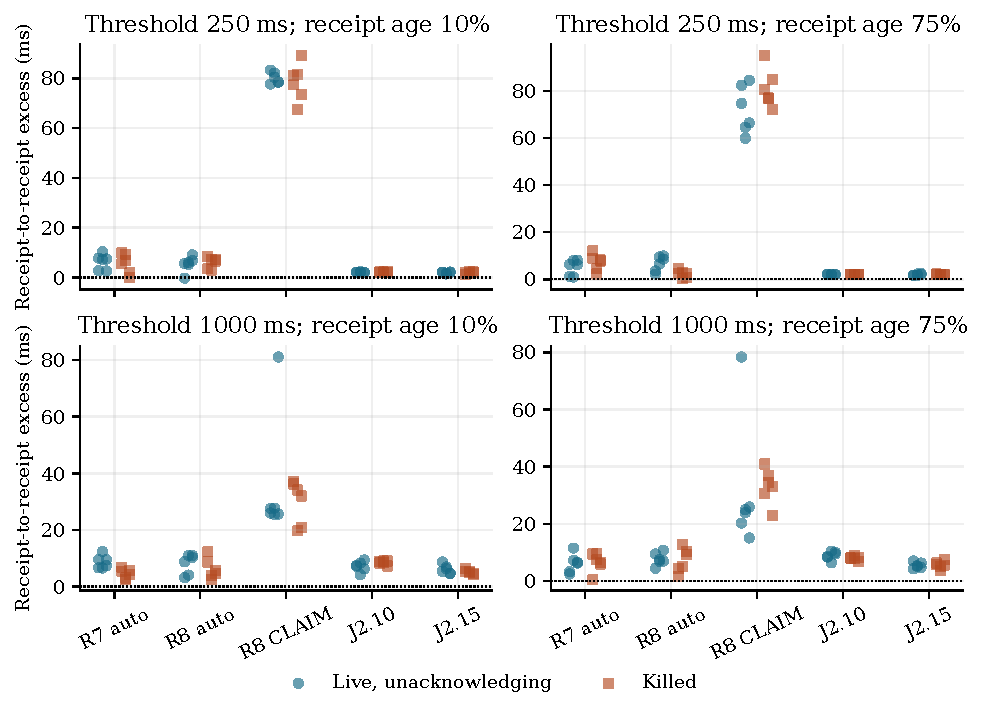
\includegraphics[width=\linewidth]{figures/followup-recovery.pdf}
\caption{Every active follow-up recovery episode, showing receipt-to-receipt time minus the configured eligibility threshold. Blue circles are live, deliberately unacknowledging victims; orange squares are killed victims. Horizontal offsets separate deployments and do not encode time. R7/R8 denote Redis 7.4.2/8.10.2; auto denotes XAUTOCLAIM with a 10 ms sleep; J denotes JetStream. Zero is a client-receipt reference, not a verified broker-side lower bound.}
\label{fig:followup-recovery}
\end{figure}

\subsection{RQ2: consumer scaling and driver capacity}

All 96 follow-up drains completed. Across deployment-specific paired comparisons, sixteen consumers raised mean throughput by 10.43--14.49 times relative to one consumer in the current memory/periodic profiles. Mean trial cycle p99 increased in all eight engine/profile/driver-quota conditions. The 65536-message drains lasted 1.77--30.11 s, extending the shortest high-concurrency observations beyond the original subsecond runs while remaining finite workloads.

At sixteen consumers, changing the driver from two to four CPUs, with matching GOMAXPROCS, produced mean paired throughput ratios of 1.031/1.026 for Redis memory/periodic and 1.107/1.102 for JetStream. Redis-periodic deployment ratios ranged from 0.993 to 1.048, so the direction was not uniform. No driver or broker cgroup throttling was recorded within the 96 bracketing drain samples. The increased rates and changed cycle tails nevertheless show that absence of throttling alone cannot establish that driver configuration is irrelevant. Table~\ref{tab:followup-drain} reports the corresponding CPU use; these observations concern the combined client, protocol and broker path.

\begin{table}[htbp]
\centering\small\setlength{\tabcolsep}{3pt}
\begin{tabular}{llrrrlrr}
\toprule
System & Mode & CPU & $X_1$ & $X_{16}$ & $X_{16}/X_1$ & Driver & Broker\\
\midrule
Redis & M & 2 & 2.83 & 34.98 & 12.36 [12.02, 12.86] & 1.08 & 0.56\\
Redis & M & 4 & 2.85 & 36.05 & 12.68 [12.21, 13.52] & 1.43 & 0.56\\
Redis & P & 2 & 2.59 & 28.55 & 11.05 [10.43, 11.73] & 0.98 & 0.64\\
Redis & P & 4 & 2.55 & 29.31 & 11.48 [11.34, 11.61] & 1.32 & 0.64\\
JetStream & M & 2 & 2.28 & 29.54 & 12.98 [12.62, 13.34] & 1.11 & 1.29\\
JetStream & M & 4 & 2.28 & 32.67 & 14.32 [14.14, 14.49] & 1.50 & 1.35\\
JetStream & P & 2 & 2.26 & 28.70 & 12.72 [12.61, 12.79] & 1.11 & 1.28\\
JetStream & P & 4 & 2.28 & 31.62 & 13.89 [13.84, 14.00] & 1.47 & 1.34\\
\bottomrule
\end{tabular}

\caption{Current-release drain results. CPU is the driver's configured quota; $X_1$ and $X_{16}$ are throughput in kmsg/s. Point values equally weight campaign means. The speedup column gives the mean and range of campaign-specific paired ratios. Driver/Broker are mean CPU cores used during the bracketing samples at $C=16$, not percentages. M/P denote memory/periodic.}
\label{tab:followup-drain}
\end{table}

\subsection{RQ3: confirmed publication from fresh stores}

At sixteen publishers, equal-weight deployment means for Redis 8.10.2 were 73.26, 60.49 and 4.35 kmsg/s in memory, periodic and always profiles. JetStream 2.15.0 yielded 60.62, 49.75 and 0.565 kmsg/s. Each condition completed all nine planned trials except JetStream always, with eight completions. The paired periodic/memory ratios averaged 0.8257 for Redis and 0.8207 for JetStream, with deployment ranges 0.8082--0.8397 and 0.8091--0.8296; all nine pairs were available in each comparison. These are configured confirmation costs from the specified starting procedure.

The latency trade-off remains visible. For memory, periodic and always profiles, respectively, mean trial p99 at sixteen publishers was 0.470, 0.563 and 16.98 ms for current Redis, and 0.639, 0.796 and 295.64 ms for current JetStream. A retained JetStream-always trial, main03/F0039, contained 976 confirmations and a 1968.6 ms p99, with nine higher order-statistic positions. Its tail remains part of the result. Appendix~\ref{app:followup} reports every condition's completion and sample counts; these empirical tails do not establish stable production percentiles.

Long requests also occurred in completed trials. Seven completed always-profile trials had a confirmed-request maximum of at least 1000 ms, spanning both brokers and both versions. Four exceeded 2000 ms, with maxima from 2.297 to 4.183 s; the next-highest maximum was 1.969 s. Appendix~\ref{app:request-maxima} lists all seven cases. These thresholds are post-observation descriptive summaries, not prospective exclusion rules or production tail guarantees. Together with the timeout outcomes, they show operationally material latency variation that is not represented by completed-run mean throughput alone.

Matched publication durations clarify the concurrency comparison that the original serial sensitivity could not isolate. For current Redis always mode, the mean paired sixteen/one-publisher ratio was 9.41, ranging from 6.06 to 13.67 across deployments, using six of nine planned pairs. Current JetStream's corresponding mean was 1.55, ranging from 0.73 to 2.46, using seven pairs. More publishers therefore did not improve every deployment's always-mode mean. Neither current release nor fresh storage removes all observed long requests or timeout outcomes. Across the eight memory/periodic version contrasts at one and sixteen publishers, equal-weight means of the deployment-specific current/historical ratios ranged from 0.9603 to 1.0232, within approximately 4\% of unity. Individual deployment ratios ranged more widely, from 0.9401 to 1.1237. All contrasts used nine completed pairs except JetStream periodic at one publisher, with eight. Appendix~\ref{app:version-contrasts} gives the individual condition summaries. These descriptive comparisons do not establish version equivalence.

\begin{figure}[htbp]
\centering
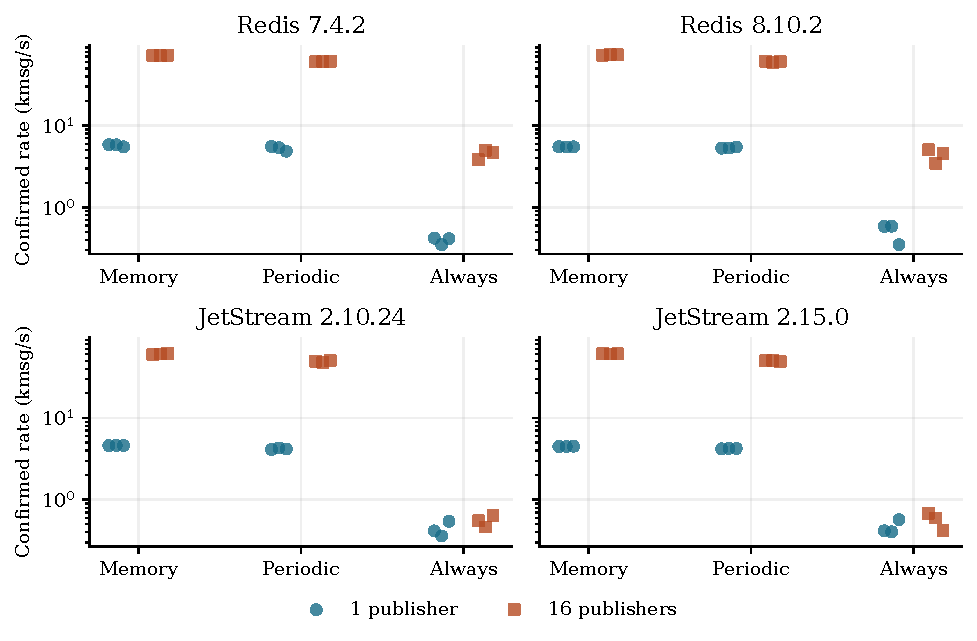
\includegraphics[width=\linewidth]{figures/followup-publication.pdf}
\caption{Fresh-store publication with matched 15-second admission budgets. Each point is one deployment's mean over completed planned trials of that condition. Horizontal offsets separate deployments; they have no quantitative meaning. The vertical scale is logarithmic. Failure counts and all per-deployment values accompany the results in Appendix~\ref{app:followup}.}
\label{fig:followup-publication}
\end{figure}

\subsection{Synchronization and compression diagnostics}\label{sec:followup-diagnostics}

All 24 trace-family and 24 compression-family trials completed. In the twelve instrumented trials, the broker-side phase brackets contained no synchronization-call errors or boundary-overlapping calls. The synchronization-call/confirmation ratio was 1.000 for current Redis with one publisher and approximately 0.120 with sixteen. Current JetStream's ratio was 1.000 at both publisher counts. JetStream's one-call-per-confirmation count at both publisher counts is consistent with serialized per-message synchronization in the tested single-stream append path: the pinned file store holds its write lock while storing a message, and its always-mode flush invokes synchronization before returning~\cite{nats2150filestore}. Redis's concurrent aggregate ratio corresponds to approximately 8.3 confirmations per synchronization call, supporting shared synchronization across publications. This identifies a source-consistent contributor to the different concurrency response; it does not assign every confirmation to an individually traced call, measure physical device flushes, or decompose the entire cross-system performance gap.

Tracing reduced throughput. Mean traced/plain ratios at one and sixteen publishers were 0.943 and 0.815 for Redis, and 0.920 and 0.934 for JetStream, respectively. Within-trace call p99 values ranged from 2.00 to 2.76 ms, and the largest traced synchronization call lasted 544.6 ms. These separate diagnostic samples did not capture the untraced primary timeout events or main03/F0039's much larger request tail, and they do not establish the cause of those events.

Disabling inherited compression produced mean off/inherited ratios of 1.036/0.995 for Redis filler/template payloads and 1.021/0.988 for JetStream. All twelve deployment-specific ratios lay between 0.935 and 1.063, with both directions represented. The complete table is in Appendix~\ref{app:followup}. This sensitivity does not support attributing the large always-mode gap to compression alone; it does not establish that compression or Btrfs is irrelevant under other conditions.

\begin{table}[htbp]
\centering\footnotesize\setlength{\tabcolsep}{3pt}
\begin{tabular}{lrllllr}
\toprule
System & $P$ & Sync calls & Calls/msg & Call p99, ms & Traced/plain & $n_t/n_p$\\
\midrule
Redis & 1 & 8327 [8233, 8427] & 1.000 [1.000, 1.000] & 2.31 [2.23, 2.42] & 0.94 [0.91, 0.97] & 3/3\\
Redis & 16 & 7349 [7270, 7392] & 0.120 [0.120, 0.121] & 2.51 [2.24, 2.76] & 0.82 [0.79, 0.84] & 3/3\\
JetStream & 1 & 7797 [7728, 7860] & 1.000 [1.000, 1.000] & 2.48 [2.23, 2.66] & 0.92 [0.90, 0.96] & 3/3\\
JetStream & 16 & 9644 [9481, 9762] & 1.000 [1.000, 1.000] & 2.33 [2.00, 2.60] & 0.93 [0.92, 0.95] & 3/3\\
\bottomrule
\end{tabular}

\caption{Current always-profile synchronization diagnostics. Entries give the mean and range of available deployment estimates; $n_t/n_p$ counts complete traces/paired comparisons, each out of three. Call p99 is a within-trace order statistic. Traced/plain is the paired throughput ratio. Counts combine fsync and fdatasync inside the broker's phase brackets; they are not physical device-flush counts.}
\label{tab:followup-trace}
\end{table}


\FloatBarrier



\section{Discussion}\label{sec:discussion}

\subsection{Recovery is a joint broker/client policy}

A recovery interval should be interpreted against message age, not simply against the full configured timeout. Equation~\ref{eq:residual} separates residual eligibility from selection and observation. Redis's current CLAIM option changes how an application requests reclamation; it does not make plain new-message reads reclaim another consumer's pending work. JetStream tracks expiry but still needs pull demand. Redelivery of live, unacknowledging work is therefore compatible with both policies. A shorter timeout can reduce waiting while increasing the risk of overlapping attempts when application processing exceeds it. Idempotency and external-effect coordination remain application concerns.

Redis's integrated CLAIM path checks pending-entry eligibility during event-loop processing. With little other activity, the default cron frequency supplies a nominal 100 ms wake-up interval; socket events can wake the loop earlier~\cite{redis8102stream,redis8102scheduling}. Eligibility checks, blocking-read timeout handling, and client reissuance can therefore contribute to receipt timing. The experiment does not instrument those internal events, so it cannot assign the observed excess to a particular scheduling component or establish an intrinsic ranking between reclamation commands.

\subsection{Concurrency gains and acknowledgment cost}

More consumers overlap request and acknowledgment waits, but can also increase cycle cost. Equation~\ref{eq:occupancy} explains why throughput and per-cycle latency can rise together. CPU telemetry and the matched driver-quota sensitivity test the available client capacity in this workload. They cannot identify an implementation-independent broker ceiling: allocation, protocol parsing, network traffic and client-library behavior remain part of the path.

The source-level acknowledgment distinction is central. JetStream's asynchronous consumer-state path prevents interpreting its fast always-profile drain acknowledgments as an equal-guarantee comparison with Redis's always-mode AOF path for group mutations. This is a semantic limit on the comparison, not a measured decomposition of its throughput gap. Publication costs are measured separately, and the current-version append error-handling difference is stated explicitly.

\subsection{What the durability comparison supports}

Fresh processes and stores remove the known cross-trial AOF/store accumulation in the follow-up. Matching duration and publisher count also makes its concurrency contrasts interpretable as changes within that defined procedure. The original campaign remains informative about its own accumulated-storage conditions. Its difference from the follow-up is not a reset-only intervention: duration, resource limits and other procedures also changed.

Synchronization traces describe completed software calls and their observed durations; matched untraced trials expose tracing overhead. These separate diagnostic trials cannot retrospectively trace the original incidents or the untraced primary failures. Compression-policy sensitivity tests one potential contributor on the same Btrfs device. Neither establishes that Btrfs is the dominant cause of always-mode costs, nor that each call corresponds to a distinct device flush. Such attribution would require additional controls and storage instrumentation. No publication latency, successful readback or consumer kill establishes the stable-media state after a power failure.

\section{Threats to validity}\label{sec:validity}

\paragraph{Construct validity.}
Reliability means observed identities, confirmations, pending-state reconciliation and recovery in the specified consumer-fault model. Stored-payload readback strengthens the follow-up integrity check but does not compare every delivered payload inside the timed drain. Neither campaign tests exactly-once business effects, replicated consensus or storage-fault durability. Client receipt differs from broker delivery, and the killed-consumer reference event has a measured invocation/exit bracket.

\paragraph{Internal validity.}
Both nodes host unrelated services. CPU limits, randomization, fresh stores and phase counters do not remove shared-device load, caching, allocation history, network variation or thermal effects. The common warm-up has product-specific physical effects. Fresh broker processes prevent concurrent follow-up broker workloads, but other host activity remains. The original campaign's large unre-written AOF is a documented carryover confound. Follow-up storage reset removes that specific accumulation; comparisons between the two campaigns cannot isolate its effect.

\paragraph{Measurement validity.}
Different client libraries and protocols remain part of the measured system. Closed-loop publication omits delays that an externally scheduled arrival process could impose. Fifteen-second windows and finite backlogs do not establish stationarity or saturation. Cgroup sample windows bracket rather than exactly equal request windows; broker-container CPU includes control and tracing processes. Syscall tracing perturbs execution. Compression flags specify policy, not the compression ratio of every extent. Requests lost through abrupt driver failure before serialization remain an unclosed recording boundary.

\paragraph{Statistical conclusion validity.}
Original bootstrap intervals depend on nine or ten completed trials and a working block-resampling model. Failure-associated missingness, serial dependence and influential tails are not repaired by more resamples. Follow-up results report three separately provisioned campaigns on the same hardware, not independent hosts, verified confidence coverage or external replication. Their ranges express observed between-campaign variation, not prediction intervals. Per-condition and paired-completion counts accompany estimates. Small empirical p99 samples remain descriptive order statistics; historical D040's p99 is the second-largest of 149 observations.

\paragraph{External validity.}
The study uses one Btrfs/NVMe environment, single replicas, 512-byte payloads, at most sixteen workers and a fixed pair of client libraries. The pseudorandom sensitivity retains a finite repeating template bank. There is no second filesystem, open-loop load, application-processing workload, large pending set, saturated recovery, geographic distribution, quorum fault or power-cut experiment. Current releases are current as of the stated review date, not indefinitely. The literature review is targeted and makes no exhaustive novelty claim.

\section{Artifact availability and reproducibility}\label{sec:artifact}

The public repository is \url{https://github.com/vicotrbb/redis-jetstream-reliability}. The retained version~1.1.0 release preserves the preceding manuscript and evidence. Version~1.2.0 contains the main article and supplement, raw compressed timings, plans, failure/development records, environment and binary receipts, pinned source references, analysis, figures, and the selected Lean model. Original manuscript, data and narrative material use CC-BY-4.0; original software and formalization use MIT. \artifact{LICENSE.md} defines third-party exceptions. No DOI assignment or peer-reviewed publication is claimed.

Offline reanalysis checks original evidence against its frozen inventory and verifies each follow-up campaign's input, invocation, environment and raw-data records. It reconstructs IDs, counts, intervals, throughput, order statistics, paired contrasts, CPU deltas and synchronization summaries. The original and follow-up datasets remain separate. D038's missing client observations and historical censor endpoints remain unavailable. New collection requires new identities and destinations; failed attempts cannot be overwritten or automatically replayed.

Release manifests bind the exact source, main PDF, supplement, analysis and rendered document QA. The builder refuses version reuse and verifies a fresh archive extraction. Hashes establish consistency of supplied bytes, not independent certification of collection time or completeness. Public access and computational reproduction are distinct from an external experimental replication or an independent artifact evaluation.

OpenAI Codex assisted with source investigation, software, analysis, formalization, drafting and internal checking. Scientific claims are grounded in cited primary sources, stated assumptions and retained measurements. AI-assisted internal review is not independent scientific peer review, and no generated benchmark value substitutes for an observation.

\section{Conclusion}\label{sec:conclusion}
This study evaluated Redis Streams 7.4.2 and NATS JetStream 2.10.24 through explicit protocol analysis, conditional mathematical proofs, selected machine-checked model results, and retained homelab measurements. Its conclusions are bounded by single-replica deployments, the specified client paths, compressible 512-byte payloads, and one shared storage environment.

For RQ1, observed failure-to-redelivery intervals were consistent with the remaining eligibility timeout and subsequent recovery scheduling. Later kills were followed by shorter intervals in both systems, and longer Redis reclaim sleeps were associated with longer additional delays. All ten new-read-only controls remained pending. All 120 active recovery episodes completed with the original identifier and cleared pending state. The residual-time theorem explains this pattern under stated timing assumptions. Neither the observations nor the theorem establish death detection or guaranteed empirical deadlines.

For RQ2, mean acknowledged backlog-drain throughput with sixteen logical consumers was 8.59--12.94 times the one-consumer mean across profiles. Cycle p99 was higher while the backlog completed sooner. The verified finite-window occupancy conditions and the identity $X=CU/\overline R$ connect this sublinear scaling to the measured cycle cost. They do not establish an unbounded scaling law, and the different always-mode consumer-state persistence paths prevent interpreting that cross-system drain comparison as equal-guarantee performance.

For RQ3, periodic configurations had approximately 83\% of Redis memory-mode publication throughput and 82\% of JetStream memory-mode throughput. Always-mode publication exhibited lower throughput and greater variability, including one failed planned Redis trial. Completed-run means and nominal intervals retain that conditioning; the failure and operational deviations remain visible. Leave-one-block-out diagnostics preserve the directions of paired contrasts, while influential observations, sparse tail information, execution-order variation, and unequal storage-history carryover limit precision and prevent isolating synchronization-policy effects. The separate serial sensitivity further shows why duration and request concurrency must accompany a throughput figure. No consumer-kill or publication-latency result establishes power-loss durability.

The contribution is an auditable, computationally reproducible comparison of specific recovery policies, concurrency behavior, and acknowledgment costs under documented conditions. The versioned, licensed artifact traces numerical claims to retained observations and formal claims to their premises. Future work should repeat the study across independent storage hosts and less-compressible payloads, hold duration fixed while varying publication concurrency, and add replication, large pending sets, open-loop load, and controlled broker/storage faults. These extensions would address external validity and failure classes that the present evidence leaves unresolved.


\appendix
\section{Complete concurrency matrix}\label{app:matrix}
The supplement's complete original concurrency matrix retains all thirty conditions, each with ten trials and 16384 messages. It reports trial-mean throughput with nominal bootstrap intervals and distinguishes cycle p99 from common-drain-start-to-receipt p99. The follow-up matrix separately reports each deployment, driver quota, concurrency and persistence profile. Machine-readable trial and condition summaries accompany both matrices in the artifact.

\section{Serial-publisher sensitivity}\label{app:serial}
The supplement retains the original serial table: one publisher, one outstanding request, 1024 messages per trial and ten randomized blocks. That fixed-count experiment differs in duration from the original five-second concurrent workload. The follow-up instead compares one and sixteen publishers under the same 15-second admission budget, with completion counts and paired estimates reported separately.

\section{Formal assumptions and claim-to-evidence map}\label{app:evidence}
\begin{longtable}{L{.20\linewidth}L{.33\linewidth}L{.36\linewidth}}
\toprule
Claim & Evidence & Boundary\\
\midrule\endhead
Residual recovery delay & Equation~\ref{eq:residual}; fault/reference timestamps & Requires retained state and explicit finite selection/demand-delay bounds\\
No new-read reclamation & Model counterexample; plain-read controls; pinned Redis source & Specific to plain new-message reads without reclamation\\
Concurrency cost & Equation~\ref{eq:occupancy}; original and follow-up drain traces & Finite workload and measured client path; no universal monotonic scaling claim\\
Persistence cost & Original publication/serial outcomes; fresh-store campaigns; matched durations and traces & Confirmation and configured policy, without power-loss or I/O-fault validation\\
Stable-storage implication & Conditional storage argument and full supplementary proof & Abstract successful-and-honored synchronization contract; no implementation verification\\
Application effect ambiguity & Two-order crash counterexamples and supplementary proof & Separate non-idempotent effect and acknowledgment; not an impossibility result for transactional applications\\
Observed identities & ID/count checks; follow-up full stored-payload readback & Historical checks are narrower; readback is not a storage-fault test\\
\bottomrule
\end{longtable}

\clearpage
\begingroup\raggedright
\bibliographystyle{plainurl}
\bibliography{references}
\endgroup
\end{document}
